
\documentclass[11pt]{article} 


%%% PACKAGES
\usepackage{multirow}
\usepackage{graphicx}
\usepackage{amsmath}
\usepackage{amsfonts}
\usepackage{bm} % for bold math terms
\usepackage{booktabs} % for much better looking tables
\usepackage{array} % for better arrays (eg matrices) \in maths
\usepackage{paralist} % very flexible & customisable lists (eg. enumerate/itemize, etc.)
\usepackage{verbatim} % adds environment for commenting out blocks of text & for better verbatim
%\usepackage{subfig} % make it possible to include more than one captioned figure/table \in a single float
\usepackage{accents} % for under-letter accents
\usepackage{float}
\usepackage{caption}
\usepackage{subcaption}
\usepackage{epstopdf}
\usepackage{tikz}
\usetikzlibrary{arrows,positioning,shapes.geometric}
\newcommand*{\figuretitle}[1]{%
    {\centering%   <--------  will only affect the title because of the grouping (by the
    \textbf{#1}%              braces before \centering and behind \medskip). If you remove
    \par\medskip}%            these braces the whole body of a {figure} env will be centered.
}



%\usepackage{Sweave}
%
%\SweaveOpts{concordance=TRUE}
%

\usepackage[top=0.5in, bottom=0.5in, left=0.5in, right=0.5in]{geometry}

%%% HEADERS & FOOTERS
\usepackage{fancyhdr} % This should be set AFTER setting up the page geometry
\usepackage[square,numbers]{natbib}
\usepackage{amsmath}

\pagestyle{fancy} % options: empty , plain , fancy
\renewcommand{\headrulewidth}{0pt} % customise the layout...
\lhead{}\chead{}\rhead{}
\lfoot{}\cfoot{\thepage}\rfoot{}

%%% SECTION TITLE APPEARANCE
\usepackage{sectsty}
\allsectionsfont{\sffamily\mdseries\upshape} % (See the fntguide.pdf for font help)
\newcommand{\sect}[1]{\section*{#1}\addcontentsline{toc}{section}{#1}}
\newcommand{\subsect}[1]{\subsection*{#1}\addcontentsline{toc}{subsection}{#1}}
\newcommand{\subsubsect}[1]{\subsubsection*{#1}\addcontentsline{toc}{subsubsection}{#1}}

%%% ToC ( contents) APPEARANCE
\usepackage[nottoc,notlof,notlot]{tocbibind} % Put the bibliography \in the ToC
\usepackage[titles,subfigure]{tocloft} % Alter the style of the Table of Contents
\renewcommand{\cftsecfont}{\rmfamily\mdseries\upshape}
\renewcommand{\cftsecpagefont}{\rmfamily\mdseries\upshape} % No bold!

%%% END Article customizations
\DeclareMathOperator*{\argmax}{arg\,max}
\DeclareMathOperator*{\argmin}{arg\,min}
\newcommand{\utilde}[1]{\underaccent{\tilde}{#1}}

\title{Predicting the Connectome Using Calcium Fluorescence Data}
\author{Guy W. Cole, Isaiah S. Morales, Austin Stone}
%\date{21 Sept. 2012} % Activate to display a given date or no date (if empty),
         % otherwise the current date is printed 

\begin{document}

\maketitle

\tableofcontents

% \newpage


\begin{center}
\textbf{
\section{What is the Connectome and Why Do We Care?}}
\end{center}

Connectome is a term used to describe the interconnectivity between neurons; it can be thought of a directed graph which maps the axonal connections between neurons.  In the directed graph, the weights of edges represent how likely a spike in the parent node is to cause a spike in the child node. 

\begin{figure}[H]
\centering
\figuretitle{The Connectome as a Directed Graph}
 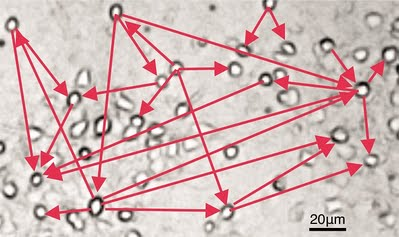
\includegraphics[width = 3in]{connectivity.jpg}
\caption{This image shows a hypothetical mapping of the connectome for a group of neurons. The neurons themselves are easily visible under microscope, but the connections between neurons are much harder to detect.}
\end{figure}

Understanding the connectivity between neurons is important for several reasons. Firstly, biological systems systems can offer insight and inspiration for new computational techniques and neuromorphic systems which can help extend the capabilities of artificial intelligence. Understanding the connectome gives us a much better understanding of how biological systems "compute" and store information, which in turn can be used to develop more biologically inspired computation techniques and hardware.


Another important reason for understanding the connectome is that it could give us greater insight into many pathologies which affect the brain. Alterations in brain structure associated with neurological diseases such as epilepsy and Alzeimer's could likely be much better understood if we could successfully and efficiently map the connectome.  


Furthermore, the ability to map the connectome would help us acquire a greater understanding of biological intelligence in general. The problem of inferring the connectome represents one of the main barriers in to making progress toward answering some of the major questions in neuroscience, e.g., how do brain states arise, how does the brain encode information, and how can conscious experience be explained rigorously in terms of neurological behavior? 

Neuroscientist Patric Hagman said the following about the connectome in his Ph.D thesis: 

"It is clear that, like the genome, which is much more than just a juxtaposition of genes, the set of all neuronal connections in the brain is much more than the sum of their individual components. The genome is an entity it-self, as it is from the subtle gene interaction that [life] emerges. In a similar manner, one could consider the brain connectome, set of all neuronal connections, as one single entity, thus emphasizing the fact that the huge brain neuronal communication capacity and computational power critically relies on this subtle and incredibly complex connectivity architecture." \cite{Hagmann}

 
 
 \begin{center}
 \textbf{
\section{The Connectomics Competition}}
\end{center}



Kaggle is a website that sponsors data mining and machine learning competitions. Kaggle receives data from companies and researchers and opens challenges to programmers, data miners and statisticians around the world to compete to produce the best models. Kaggle challenges effectively crowdsource statistical and big data related problems that don't currently have canonical solutions.


The challenge that motivated this project (titled CONNECTOMICS on Kaggle) was to provide the most accurate connectome of a population of neurons given each neuron's position and fluorescence data over a period of an hour. The neurons span a circumference of 1 mm of two dimensional space, and the positional coordinates are given in units of mm. The fluorescence data is a measure of neural activity. Fluorescence data is recorded by placing a fluorescence probe on each neuron that optically measures chemically indicated calcium molecules at a sampling rate of 50 Hertz. Whenever a probed neuron fires, the amount of extracellular calcium rises which is in turn recorded by the probe. This is a common laboratory technique to monitor the activity of tens of thousands of neurons simultaneously. 


This sort of data is typical and not difficult to acquire; it is easy to visually locate all neurons on a petri dish and monitor their activity, but it is currently intractable to directly determine which neurons have axons connecting them to other neurons. Thus, a current outstanding problem in neuroscience is to infer the connectome indirectly. The approach that the Kaggle challenge presumes is to infer the connectome via correlations in the fluorescence data.
\begin{figure}[H]
\centering
\figuretitle{Correlations in Fluorescence Data}
 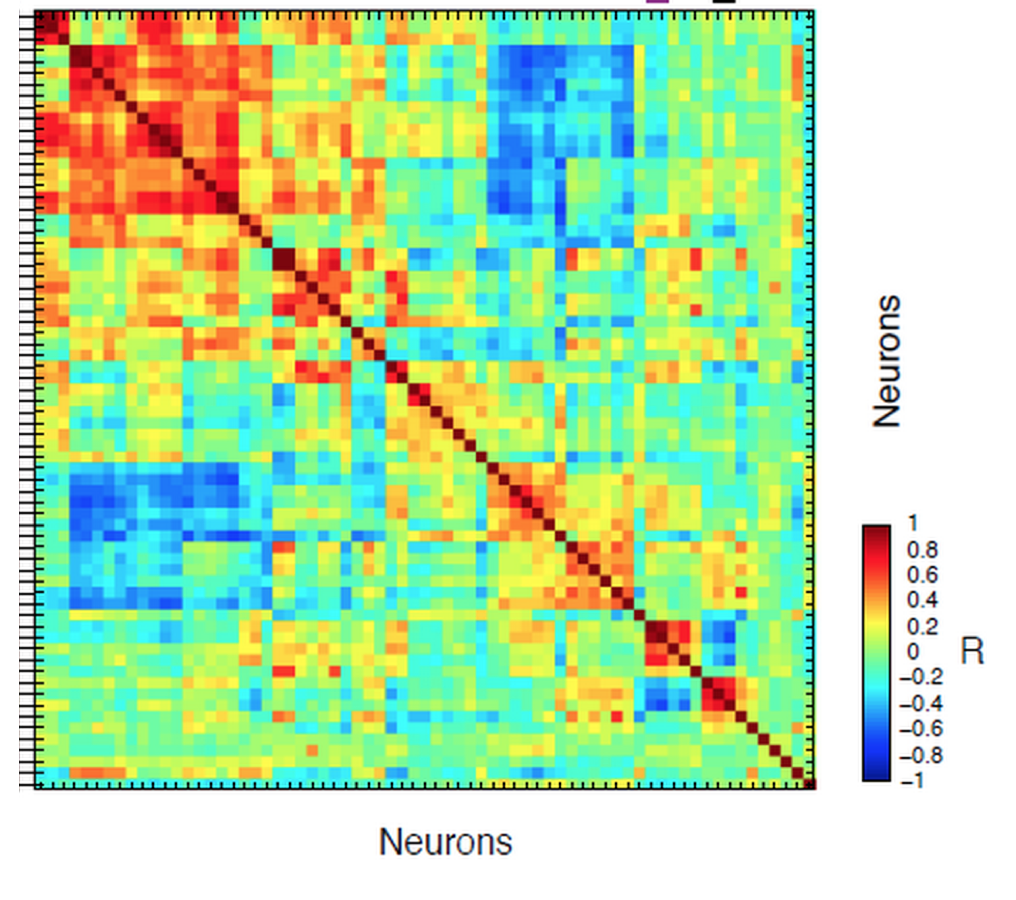
\includegraphics[width=3in]{correlatedNeurons.png}
\caption{Here is an example map of the correlation coefficients between 100 neurons. A high correlation coefficient between two neurons can mean that there exists an axonal connection between them.}
\end{figure}



\begin{center}
\textbf{
\section{Difficulties in Inferring the Connectome}}
\end{center}
 
 
 
   
	A neuron's fluorescence values affect the fluorescence of other nearby neurons even if they are not connected due light scattering effects. Blurring linearly combines the true fluorescence value of a neuron with the fluorescence values of its neighbors. This causes nearby neural fluorescence data to look more similar than it should, and it can cause confusion as to which neuron is actually responsible for the fluorescent output. 

\begin{figure}[H]
        \centering
        \begin{subfigure}[b]{0.5\textwidth}
                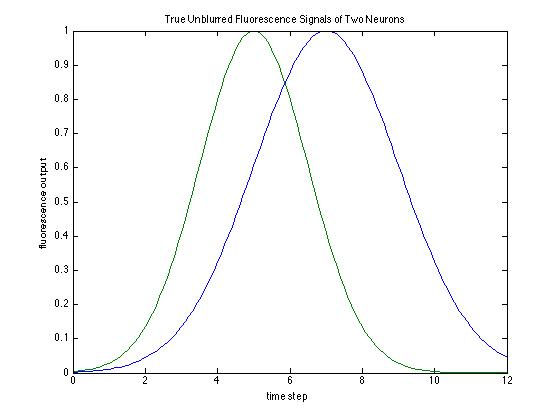
\includegraphics[width=\textwidth]{two_unblurred_neurons.jpg}
                \caption{"True" unblurred fluorescence patterns from two different but spatially close neurons. Note that the actual fluorescence signal is discretized, as discussed below.}
                \label{fig:unblurred}
        \end{subfigure}%
        ~ %add desired spacing between images, e. g. ~, \quad, \qquad etc.
          %(or a blank line to force the subfigure onto a new line)
        \begin{subfigure}[b]{0.5\textwidth}
                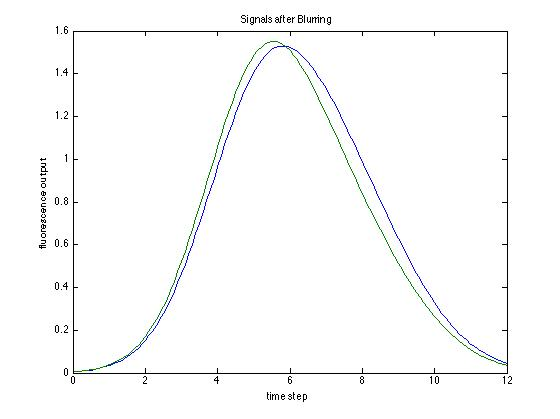
\includegraphics[width=\textwidth]{blurred_fluorescence.jpg}
                \caption{Blurred fluorescence pattern from the same two neurons. The discretized version of this is what would actually be picked up by the probes.}
                \label{fig:tiger}
        \end{subfigure}
      \end{figure}
   




  The fluorescence data is sampled in intervals of 20 ms, which is often slower than neural firing which can happen as quickly as every 5 ms. The rate of sampling is too slow to infer exactly when spikes happen and likewise to naively infer which spikes caused other spikes. Furthermore, the slow rate of sampling and slow rate of fluorescence decay can present a problems both in terms of saturation (i.e., the fluorescence imaging reaches the maximum recording threshold during periods of fast spiking and information is lost) and in terms of identifying when spikes actually happen, since simple thresholding will not work to determine when spikes occur. 



\begin{figure}[H]
        \centering
        \begin{subfigure}[b]{0.5\textwidth}
                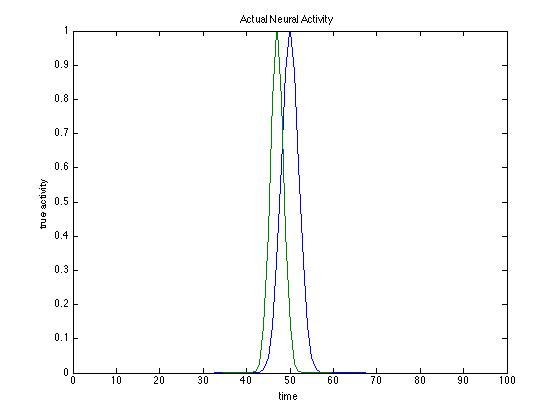
\includegraphics[, width=\textwidth]{true_activity.jpg}
                \caption{This is an example of the true neural activity in terms of membrane potential.  Y-axis is arbitrary units.}
                \label{fig:unblurred}
        \end{subfigure}%
        ~ %add desired spacing between images, e. g. ~, \quad, \qquad etc.
          %(or a blank line to force the subfigure onto a new line)
        \begin{subfigure}[b]{0.5\textwidth}
        \centering
                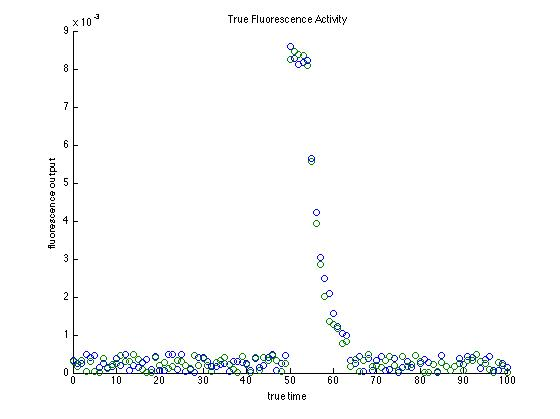
\includegraphics[ width=\textwidth]{fluorescent_timestep_problem.jpg}
                \caption{Actual fluorescence reading for the same Acitivity pattern in part (a). Y-axis is arbitrary units. }
                \label{fig:tiger}
        \end{subfigure}
      \end{figure}
   
   
   The slow rate of sampling in conjunction with fluorescence blurring renders many naive methods of determining connectivity untenable. Not only is it difficult to determine when exactly a spike does occur, it can be difficult to determine which neuron actually elicited that spike due to blurring. 

   % 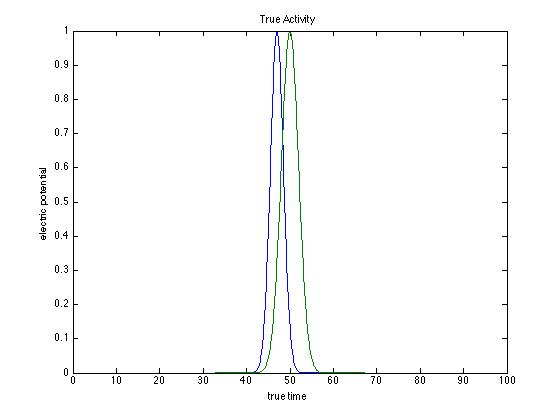
\includegraphics[width=55mm]{true_fluorescence_activity.jpg}
   
  %  \includegraphics[width=55mm]{}


\begin{center}
\textbf{
\section{Stetter 2012 \cite{Stetter} }}
\end{center}

To test the accuracy of a predicted connectome, one needs to know the actual connectome. Since determining the actual connectome is such a hard problem and consequently very few actual network connectomes are known, the Kaggle challenge uses data simulated from a virtual population of neurons in which the connectome is known via the method outlined in \textit{Model-Free Reconstruction of Excitatory Neuronal Connectivity from Calcium Imaging Signals}\cite{Stetter}. This simulation has been shown to capture the behavior of biological neurons in all meaningful aspects. 


Stetter describes the mathematics of blurring. Given the true population fluorescence vector for a time step, the blurred fluorescence vector for that time step can be acquired by multiplying the true fluorescence with the matrix $A$ where \[ A(\alpha, \lambda)_{ij} =  \alpha e^{-\frac12 \frac{ || x_i - x_j ||_2^2 }{ \lambda^2 } } + (1 - \alpha) \delta_{i=j} \]

$\alpha$ and $\lambda$ are both parameters that are determined by the typical light deflection in the medium and the optical apparatus. We incorporated this prior knowledge of the mechanics of blurring into our model, as described in the Model Details section. 


Other information from Stetter which we incorporated into our model was the latent variable of  connectivity. The connectivity constant, $p$, is the chance that two arbitrary neurons are connected to each other. This plays into our model in that it affects the prior distribution of what we believe the connectome is. 

\begin{figure}[H]
        \centering
        \begin{subfigure}[b]{0.5\textwidth}
                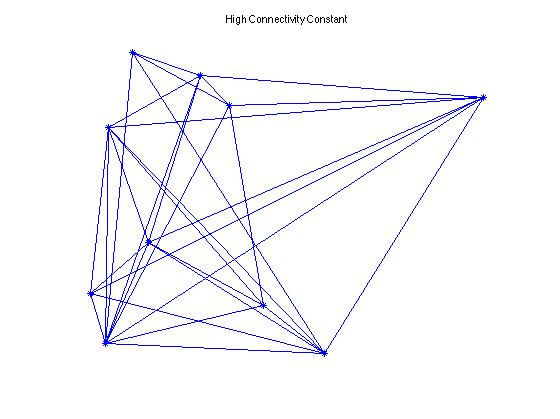
\includegraphics[, width=\textwidth]{high_connectivity_constant.jpg}
                \caption{Relative to figure b, this graph has a high connectivity constant. The chance that two nodes have a connecting edge is higher than it is in figure b. }
                \label{fig:unblurred}
        \end{subfigure}%
        ~ %add desired spacing between images, e. g. ~, \quad, \qquad etc.
          %(or a blank line to force the subfigure onto a new line)
        \begin{subfigure}[b]{0.5\textwidth}
        \centering
                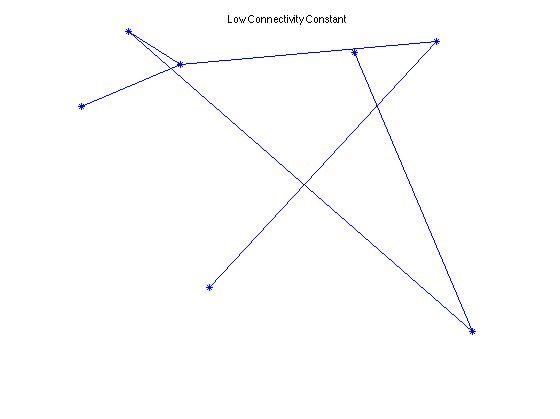
\includegraphics[ width=\textwidth]{low_connectivity_constant.jpg}
                \caption{Relative to figure a, this graph has a low connectivity constant. The chance that two nodes have a connecting edge is relatively low.}
                \label{fig:tiger}
        \end{subfigure}
      \end{figure}
   

The connectivity constant varies from population to population of neurons, and it is heavily dependent on the species and brain region which the neurons were taken from. In our model, we assumed the connectivity constant to be .12 based on the sample data we were given and the connectivity constant used in Stetter. 
    
 \begin{center}
 \textbf{
\section{High Level Overview of Our Model}}
\end{center}

Our model seeks to describe the system of differential equations identified by Stetter in a reduced space.	Because the system of equations could be arbitrarily complex (even $n^n$) it is intractable to attempt to model the complete space of possible coefficients.  Instead, we focus on first order interactions, specifically:
	
\[ F_{i,t} = \left(\begin{smallmatrix} F_{\dot,t-1} \\ F_{i,t-1} \times F_{\dot,t-1} \end{smallmatrix}\right)^T \beta_i + \epsilon_{i,t}^{\mathbb{M}}  \]

This series of looks online one time step into the past, and seeks to model the interaction of this cell with the state of each other cell; it assumes that other cells have independent effects on this cell.

The primary advantage of this model over a more complete system of interactions is that it is computationally tractable.  The fitting algorithm later scales with $O( p^3 )$, where in this case $p = 2n$, but the more complex models could be $p = Ln^n$, where $L$ is the number of time steps considered and $n$ is the number of neurons.
\begin{center}
\textbf{
\section{Model Details}}
\end{center}

Our full statistical model is:

\begin{eqnarray}
C_{ij} 	& \sim & Bernoulli( \rho ) \nonumber \\
\beta_{ij} 	& \sim & N( 0, ( \tau_1 C_{ij} + \tau_0 (1-C_{ij}) ) I ) \nonumber \\
F_{i,t}	& \sim & N\left( \left(\begin{smallmatrix} F_{\dot,t-1} \\ F_{i,t-1}F_{\dot,t-1} \end{smallmatrix}\right)^T \beta_i, \sigma_M^2 \right)\nonumber \\
F_{i,t}^{bl}	& \sim & N\left( \left( A(\alpha, \lambda) F \right)_{i,t}, \sigma_B^2 \right) \nonumber
\end{eqnarray}

Recall from Stetter that the elements of the blurring matrix are defined as:
	
\[ A(\alpha, \lambda)_{ij} =  \alpha e^{-\frac12 \frac{ || x_i - x_j ||_2^2 }{ \lambda^2 } } + (1 - \alpha) \delta_{i=j} \]

The prior of $C_{ij}$ is a simple Bernoulli prior; we believe a priori that two neurons are connected with probability of $\rho$, which is usually small (1-10\%).  The prior on $\beta_i$ acts as a spike-and-slab prior; the individual values are assumed a priori to be either from a "null" distribution heavily distributed at 0, or from a "active" distribution which is very widely distributed.  The values of $C_{ij}$ indicate which component of this mixture distribution should be drawn from.

We can sample the elements of $C$ according to their conditional posterior by evaluating the likelihood that the elements of $\beta$ corresponding to the $i,j$ relationship were drawn from either the "null" or "active" distribution, and multiplying by our prior probability $\rho$ of being active.  It is then trivial to do $MAP$ or stochastic sampling of $C_ij$.

\begin{eqnarray}
p( C_{ij} = 1 | \beta_j ) &=& \frac{ \rho N( \beta_{ij} | 0, \tau_1 ) }{ \rho N( \beta_{ij} | 0, \tau_1 ) + (1-\rho) N( \beta_{ij} | 0, \tau_0 )} \nonumber \\
odds( C_{ij} = 1 | \beta_j  ) & = & \frac{p}{1-p} = \frac{\rho}{1-\rho} \frac{\tau_1}{\tau_0} e^{-\frac12 ||\beta_{ij}||_2^2 ( \tau_1 - \tau_0 ) } \nonumber
\end{eqnarray}

$\beta$, likewise, has a multivariate Normal conditional distribution which is easy to sample from.  Note, however, that this calculation is computationally intensive: the inversion of $(\frac{1}{\sigma^2} X^T X + \tau_{C_i} I)$ scales according to the third power of the dimension of $X^TX$.  Again, it is easy to update either stochastically or using the conditional MAP estimate.  The conditional posterior is:

\[ \hat{\beta}_i | C, F  \sim  N\left( (\frac{1}{\sigma^2} X^T X + \tau_{C_i} I)^{-1} \frac{1}{\sigma^2} X^T F, ( \frac{1}{\sigma^2} X^TX + \tau_{C_i} I)^{-1} \right) \]

To update $\alpha$ and $\lambda$, we resort to random walk proposals.  However, since this computation is relatively "cheap" compared with the update of $\beta$, we choose to simultaneously evaluate many alternative pairs of $\alpha$ and $\lambda$, and then can choose either keep the MAP, keep the expectation, or simulate stochastically from the conditional posterior.
\begin{center}
\textbf{
\section{Results}}
\end{center}

We chose to evaluate our results using precision, recall, and combined F1 score.  The Connectomics competition uses a different measure\footnote{The competition uses "AUC", or "Area Under the Curve", where the "Curve" is the ROC (receive operator characteristic) curve.  Evaluation of this curve is less intuitive or meaningful for our model with several tuning paramters, and we did priority computation of a ROC curve for our results.}.  Recall that these scores are defined as:

\begin{itemize}
	\item Precision: $\frac{\text{Correct Connections} }{ \text{Total Predicted Connections} } = \frac{ TP }{ FP + TP }$
	\item Recall: $\frac{ \text{Correct Connections} }{ \text{Total True Connections} } = \frac{ TP }{ FN + TP }$
	\item F1 score: $\frac{ 2 * \text{Precision} * \text{Recall} }{ \text{Precision} + \text{Recall} }$
\end{itemize}

We used our model to predict the connectome of the training data set.  In that data set, there are 100 neurons, with 1,050 interconnections (excluding self-connections) out of a possible 9,900 (or 1,150 out of the 10,000, including self-connections).  We began with our tuning parameter $\rho$ set to $0.105$.  Below, we compare our results with those of "all connections", in which we simply set every connection to true, and "random" connections, in which we set all non-self-connections randomly with chance equal to the true rate.  The stochastic updates varied between two connection states: a "high connections" mode with better recall and lower precision, and a "low connections" mode with lower recall and better precision.

\begin{figure}
\begin{center}
\begin{tabular}{ c l l l }
Method & Pre & Rec & F1 \\ \hline
All connections & 0.115 & 1.000 & 0.206 \\
Random & 0.115 & 0.182 & 0.141 \\
Result (A) & 0.130 & 0.376 & 0.193 \\
Result (B) & 0.325 & 0.125 & 0.181 \\
\end{tabular}
\end{center}
\end{figure}

While our methodology clearly beats "naive" strategies, it does not perform particularly well in the scope of the problem.
\begin{center}
\textbf{
\section{Discussion}}
\end{center}

While our particular implementation has performed poorly, we believe this would be a valuable method of attacking the problem\footnote{Though, in retrospect, the design of the Connectomics competition seems fraught in contributing to the larger problem of estimating real-world connectomes.  Here, it is advantageous to attack the differential equations and blurring problem rather than the neuronal model.}.  Since our solution can be easily scaled to more complex models (and more complex interactions), it could eventually fully estimate the system of differential equations. The primary limiting factor is computational power; the principle tradeoff is computational time vs. model complexity.  For immediate next steps, we would suggest:

\begin{itemize}
\item A 2nd-order analysis that looks only 1 timestep back is doing a very poor job.
\item Separating the problems of deblurring and estimating the connectome would be valuable.
\item Higher-order and longer timesteps is trivial to add analytically, but computationally infeasible.
\item Algorithms are highly parallelizable (note $\hat{\beta}_i \perp \hat{\beta}_i$) so may be a good approach in need of serious computing power.
\item Incorporating knowledge of the latent variable of clustering coefficient; this dictates how tightly connected neighborhoods of nodes are. This was discussed in Stetter, but is not currently incorporated into our model. 
\end{itemize}


\begin{thebibliography}{9}
\bibitem{Stetter}
 Stetter O, Battaglia D, Soriano J, Geisel T
 \emph{ Model-Free Reconstruction of Excitatory Neuronal Connectivity from Calcium Imaging Signals}
  2012 PLoS Comput Biol 8(8): e1002653. doi:10.1371/journal.pcbi.1002653
  
  \bibitem{Hagmann}
 Hagmann, Patric
 \emph{  From diffusion MRI to brain connectomics}
 (Thesis). Lausanne: EPFL. doi:10.5075/epfl-thesis-3230. Retrieved 2014-5-5.


\end{thebibliography}



\end{document}


